\section{Study 1: User Behavior on Imaginary TypeBoard}

In this study, we collected data from participants' typing actions on a force-sensitive touchpad. The motivation was to investigate users' typing behavior on an imaginary touchscreen keyboard that can "perfectly reject unintentional touch", based on which we can design the algorithm of rejecting unintentional touch. Because (incorrect) feedback will affect users' behaviors, in this study, participants typed on a touchpad without any feedback. Participants could not enter words by typing on the touchpad, instead they imagined that the desired words are entered. Besides, participants need to adapts their typing behaviors according to the imagination that the keyboard can perfectly reject unintentional touch.

%本实验的目标是研究用户在想象中防误触键盘上的打字行为,从而指导触屏键盘防误触算法的设计。由于(不正确的)反馈可能会影响用户的输入行为,在本实验中,用户在无反馈的键盘上打字,用户不能真的键入字母,而是想象可以键入字母。另外,用户需要假想键盘可以防止误触,调整自己的打字行为。

\subsection{Participants}

We recruited 16 participants from the campus (aged from xx to xx, M = xx.xx, SD = xx.xx, xx females). All the participants were right handed and native Chinese speaker. They have used software keyboards on smartphones for not less than xx years. xx of the 16 participants were familiar with software keyboards on tablets.

\subsection{Design and Procedure}

Figure xx illustrate the experimental setting. There was a Morph Sensel [xx] force-sensitive touchpad on the desk. We placed a windows surface tablet on the touchpad, covering less than half of the pad. We drew a QWERTY layout on the touchpad using highlighter pens. This combination of touchpad and table took place of the force-sensitive touchscreen, which is expected to be commercialized in the future. Participants filled in a Microsoft Word document to complete the experimental tasks. They touched on the tablet for pointing, and typed on the touchpad to "enter words". The system recorded every touches and the screencast during the experiment.

【图:实验一的实验设置】

%图xx展示了实验的设置,桌子上放着一块morph-sensel压力触摸板,在板子的上半部分叠放了一个windows surface,我们用这个组合来模拟未来可以支持压力输入的平板电脑。用户可以根据自己的需求调整椅子的高度、压力触摸板和显示器的位置。压力触摸板上用荧光笔画上了26键Qwerty键盘布局,用于提示用户每个按键的位置。用户在这个系统中通过填写word文档的方式来完成文本输入任务,系统会记录用户每次触摸的信息,以及给实验过程录屏。

The experiment included four sessions of text entry tasks: (1) filling in personal information, (2) describing personal tastes, (3) open-book examination, and (4) picture writing. We counterbalanced the order of the four tasks using a balanced latin square. We did not include transcription as a task as many other studies of text entry do [xx,xx,xx], because our pilot study showed that participants seldom rested their fingers on the touchpad in a transcription task, resulting in low efficiency of obtaining unintentional touches. The details of the four tasks are as follows:

%实验分为四个session,分别对应四个不同的文本输入任务:填写个人信息、描述个人爱好、模拟开卷考试和看图写话。我们通过拉丁方来平衡每个用户做这四个任务的顺序。我们不像大多数文本输入相关工作一样[xx,xx,xx],将誊写作为文本输入任务,因为我们通过预实验发现,用户在誊写任务中很少将手指放在键盘上,误触的采集效率不高。图xx展示了每个任务的例子,每个任务的具体描述如下。

\begin{enumerate}
	\item{\textbf{Filling in personal information:} In the task document, there was a table of xx question about personal information, such as name, gender, and so on. Participant direct touched on the tablet to select what to fill, and typed on the touchpad the "enter words". To protect users' privacy, users were allowed to fill in fake information. This assignment represented those text entry tasks that require frequently switching between pointing and typing.}
	\item{\textbf{Describing personal tastes:} There was another table of xx question about personal tastes, such as "the favorite city", "the favorite fruit", and so on. Participant touched on the tablet for pointing and pressed on the touchpad for typing, as if they were doing office work. Participant were allowed to fill in fake information.}
	\item{\textbf{Open-book examination:} The "exam" consisted of five hard questions such as "What is the 50th element of the periodic table?". Participants could hardly know the answer, so that they needed to use the search engine. The system recorded both the behaviors of answering questions and searching in the Internet. Because the participants could not enter words in the search engine, they needed to speak out when typing, so that the experimenter could replaced them to enter the words. This assignment represented those text entry tasks that require using the search engine.}
	\item{\textbf{Picture writing:} There was a picture (as figure xx shown) in the task document. Participants needed to describe the picture in five sentences and wrote down the story in the document. We asked participants to speak out while typing, so that the experimenter could replaced the participants to enter the words. This assignment represent the text entry tasks that the users need to think while writing.}
\end{enumerate}

%\begin{enumerate}
	%\item{\textbf{填写个人信息任务:}word文档中有一个表格,其中包含用户姓名、性别、专业等问题。用户操作触摸板(想象中的TypeBoard键盘)和平板电脑上的直接触摸填写表格。为了保护用户的隐私,用户可以填写错误的信息,前提是他能记住他填写的内容,以便标注时作为参考。用户需要点击平板电脑来切换表格中的焦点,然后再触摸板上敲击“输入”,想象所需字母被填写在了word文档中。该任务模拟了真实场景中,需要频繁切换键鼠操作的输入类型。}
	%\item{\textbf{描述个人爱好任务:}word文档中有一个问卷,其中包含“最喜欢的城市”、“最喜爱的食物”等个人喜好相关的问题。和任务一相同,用户通过键鼠配合操作完成问卷的填写。该任务模拟了真实场景中简单的问卷填写任务[xx]。}
	%\item{\textbf{模拟开卷考试任务:}word文档中包含若干有一定难度的知识性问题,如“比利时的首都在哪里”、“元素周期表中第50号元素时?”。在此任务中,用户很可能不知道问题的正确答案,此时她需要通过搜索引擎来得到答案。用户在使用搜索引擎时存在一个问题是,她输入的文字并不能真的上屏,此时我们要求用户边输入边把搜索的关键词说出来,实验者帮忙使用键盘完成搜索。both搜索的过程和填写试卷的过程是本实验采集的数据。该任务模拟了真实场景中常见的搜索引擎任务。}
	%\item{\textbf{看图写话任务:}word文档中包含了一张简笔画(如图xx的xx所示),用户需要根据这幅图写一个五句话的小作文。在此任务中,我们同样要求用户边说边写,实验者在一旁进行速记,这是为了在标注中给用户提高上下文。该任务模拟了真实场景中的办公场景[xx],这一类任务有着xx的特点。}
	%\item{\textbf{誊写任务:}word文档中包含了一句话,用户需要尽可能快地将这句话誊写五次。每个用户所誊写的句子都是不同的,都是从phrase-set[xx]中随机抽取。誊写任务是文本输入工作中最常见的评测任务,适用于评测输入法的输入效率上限。}
%\end{enumerate}

Before the experiment started, the participant had five minutes to familiarize himself with the tasks and the requirements of the experiment. During the warm-up phase, the participant "typed" on the touchpad freely, while the experimenter reminded the user of two points. First, the keyboard did not provide any feedback. Participants could not enter words, but imaged that they entered words. Because the users' first language are Chinese, which involved word selection in the text entry method, users assumed that the desired word is always the first one of the candidate words. Second, users needed to imagine that the keyboard can perfectly prevent unintentional touches, and adjust their behavior according to this assumption. For example, they could rest their fingers on the keyboard while thinking. This is not mandatory. Participants could make choices as they wished.

%在实验开始前,用户有5分钟的时间自由地在本系统中熟悉实验的任务和要求,在热身的过程中,实验者让用户注意两点:第一,本实验的键盘不会提供任何反馈,用户不能键入字母,而是想象自己键入了字母。由于用户的母语是中文,在输入的过程中会涉及到选词,用户只需想象想要的单词总是在输入法候选词的第一位。第二,用户需要想象该键盘可以完美地防误触,并根据这一条件调整自己的输入行为,比如,在思考问题的时候可以将手指休息在键盘上。这种行为调整不是强制性的,用户可以根据自己的实际情况作出选择。

After finishing each session of task, the participant labeled the data through an interactive program. The program showed the capacitive images of touchpad and the screencast of tablet at the same time. As figure xx shows, there were some red points on the capacitive images that showed the touchpoints reported by the touchpad. Participants labeled the intended touches as green points. Because participants got context information from the screencast, they were able to identify most intentional touches. If participants were not sure, they could label the touchpoint as a blue point to remove the data. In average, participants spent five minutes to finish the text entry tasks and spent 45 minutes to label the data. Participants rested for five minutes between two sessions to avoid fatigue. The study was generally completed within 70 minutes.

%在每个session结束后,用户需要通过一个交互式程序来标注刚刚所进行session的报点数据,该程序同时展示了实验过程中的录屏视频和压力板图像,用户需要结合录屏提供的上下文信息,标注压力板图像中的报点。如图xx所示,我们在平板电脑上外接了鼠标来提高用户的标注效率。压力图像中所包含的报点初始默认值为负例(误触),用红色点表示。用户若认为一个报点是正例(打字事件),则需要用鼠标左键将该点标为绿色;用户可以通过鼠标右键将报点重新标为红色;用户若不清楚该报点是正例还是负例,则需要用鼠标中键将该点标为蓝色,表示剔除出数据集。本实验的输入任务部分,四个session加起来大约需要15分钟,标注过程大约45分钟,每两个session之间休息5分钟时间来避免疲劳,实验总时长为80分钟。

\subsection{Apparatus}

As figure xx shows, we placed a Windows surface tablet and a Morph Sensel force-sensitive touchpad [xx] together to simulate a tablet computer that contains force-sensitive touchscreen. The Sensel Morph is a multi-touch and force-sensitive touchpad, which sense the position and the pressure level of touches. The Sensel Morph contains 185 x 105 sensor elements ("sensels") at a 1.25mm pitch. Each contact can sense approximately 30000 levels, ranged from 5g to 5kg. The upper limit of frequency is 125Hz (8ms latency), while we slowed it down to 50Hz to fetch stable data. The Sensel Morph provides capacitive images and touchpoint information including position, timestamp, touch area, pressure level and shape. The recognition of touchpoint is sensitive that almost every contacts are reported as touchpoints, so in this paper, we identified unintentional touches among reported touchpoints, while did not consider missing touches by the Morph Sensel.

%由于目前在商业上还没有具备压力感知能力的平板电脑(或是压力信息不灵敏[xx]),我们拼接了Morph Sensel压敏触摸板和Windows Surface平板电脑来模拟未来可能普及的压敏平板电脑(如图xx所示)。Morph Sensel是一个支持多点触摸的压敏触控板,可以感知触摸的位置和力度,185 x 105 sensor elements ("sensels") at a 1.25mm pitch,5g - 5kg sensing range per touch,Each contact can sense approximately 30,000 levels。Extremely Fast:High Speed Mode: 500 Hz (2 ms latency). morph sensel触摸板在提供电容屏图像的同时,还会提供报点信息,报点十分敏感,几乎所有的contact都会视为一次报点,因此在这份工作中,我们仅分析sensel的报点中哪些是误触,而不考虑morph sensel本身漏报的情况。

【图:实验设置,特别是平板电脑+压力触控板=压敏平板电脑】

The size of sensing area on the Morph Sensel is 240mm x 138mm. We used highlighter pen to draw a Qwerty layout on the touchpad as shown in figure xx. The width of the Morph Sensel (240mm) is a little shorter than the width of the keyboard on a 15 inches MacBook (270mm). We removed some keys that are less frequently used such as square brackets and semicolon, so that the Qwerty layout could be placed in the Morph Sensel, while the size of each key reminded the same as Macbook. Because the Qwerty layout is changeable in software keyboard, we did not used the layout as prior knowledge in the recognition of unintentional touch.

%传感区域的大小是240mm*138mm,我们在传感区域中央用记号笔画上了Qwerty布局,用来提示用户每个按键所在的位置。Morph Sensel的传感区域比15寸MacBook上的键盘(xx-mm*xx-mm)小一些,为了能在触摸板上画上Qwerty布局,而不对用户的打字行为造成太大的影响,如图xx所示,我们维持了MacBook键盘上每个按键的大小,并去除了本次实验中不会用到的符号键(如中括号和分号)。由于软键盘的布局可以多种多样,而我们希望做一个应用范围更广的防误触算法,因此我们不会将键盘布局作为先验知识应用在防误触算法当中。

The tablet we used in the experiment was Windows surface xx, with ixx Intel Core Processor, xx-core. The data collecting program ran on the tablet at a stable frequency of 50 FPS.

\subsection{Result}

The dataset contains 12659 touches, excluding the ambiguous touches (0.18\%) in the labeling. 67.5\% of the data were positive samples (intentional touches), while 32.5\% were negative samples (unintentional touches). Because some participants misunderstood the concept of "unintentional touches", there might be mislabeled data points. We trained a simple machine learning model (version 1) to process the data. If there were a large between labels and predicting results, we asked the participants to relabel the suspicious data points.

\subsubsection{Model version 1: naive model and data processing}

We first trained a simple and straightforward model (version 1) for data processing. We sampled the first five frames of each touch. If the duration of a touch is shorter than five frames, the whole touch was regarded as a sample. As table xx (V1) shows, we extracted features from the samples as follows: for the contact area, ellipticity, displacement, force and intensity over frames, we calculated their temporal feature including maximum, minimum, mean, skewness and kurtosis. Then, we concatenated these values to obtain a feature of 25 dimensions and trained an SVM binary classifier. Positive and negative samples were balanced in weight.

%如表格xx所示,我们首先开发了一个简单、直观的机器学习方法(version-1)。我们采样每个报点后前5帧(100ms)的数据作为样本,如果一次点击事件的持续时间不足五帧,则将整个点击事件作为样本。然后,我们通过以下方法来提取样本的特征:对于报点面积、椭圆度、位移、压力和压强这五个数值,分别计算它们在五帧中的时序特征(最大值、最小值、平均值、偏度和峰度),排列成一个25维的特征向量,最后使用SVM二分类器进行分类,训练时平衡了正负样本的权重,也对每一维特征分别先进行归一化。

We used this model to simulate the dataset and observed. We found that some participants misunderstood the concept of "unintentional touches", for example, regarding wrong inputs as unintentional touches. We asked the participants to relabel the suspicious data points through e-mail. Finally, we had xx data points, including xx.x\% positive samples and xx.x\% negative samples.

%我们用这个简单的机器学习方法来预测实验一中采集的数据。我们发现,有的用户在标注的时候对误触的理解出现了偏差,例如将打错字母标注成无意触摸,对于这种实验者认为有可疑的数据点,我们都通过邮件的方式请当事人用户重新标注。在所有数据都被检查无误之后,我们共有xx个数据点,其中正例占xx.x\%,负例占xx.x\%。至此,我们认为数据集的标注准确无误。

Leave one out cross-validation shows that the accuracy of model version 1 was 96.86\% (SD=4.17\%). For comparison, if we did not have the force signal (i.e., the regular touchscreen devices), the accuracy would reduce to 92.30\% (SD=4.88\%). The result shows that the force signal is important for unintentional touch rejection (F,p).

%留一法显示版本1的模型对误触的识别准确率达到96.86\%,作为对比,如果我们不利用压力信息(版本0),准确率仅为92.30\%。这一结果说明,压力信号在tablet键盘防误触方面起了非常重要的作用(F,p)。

\begin{figure}[!tbh]
	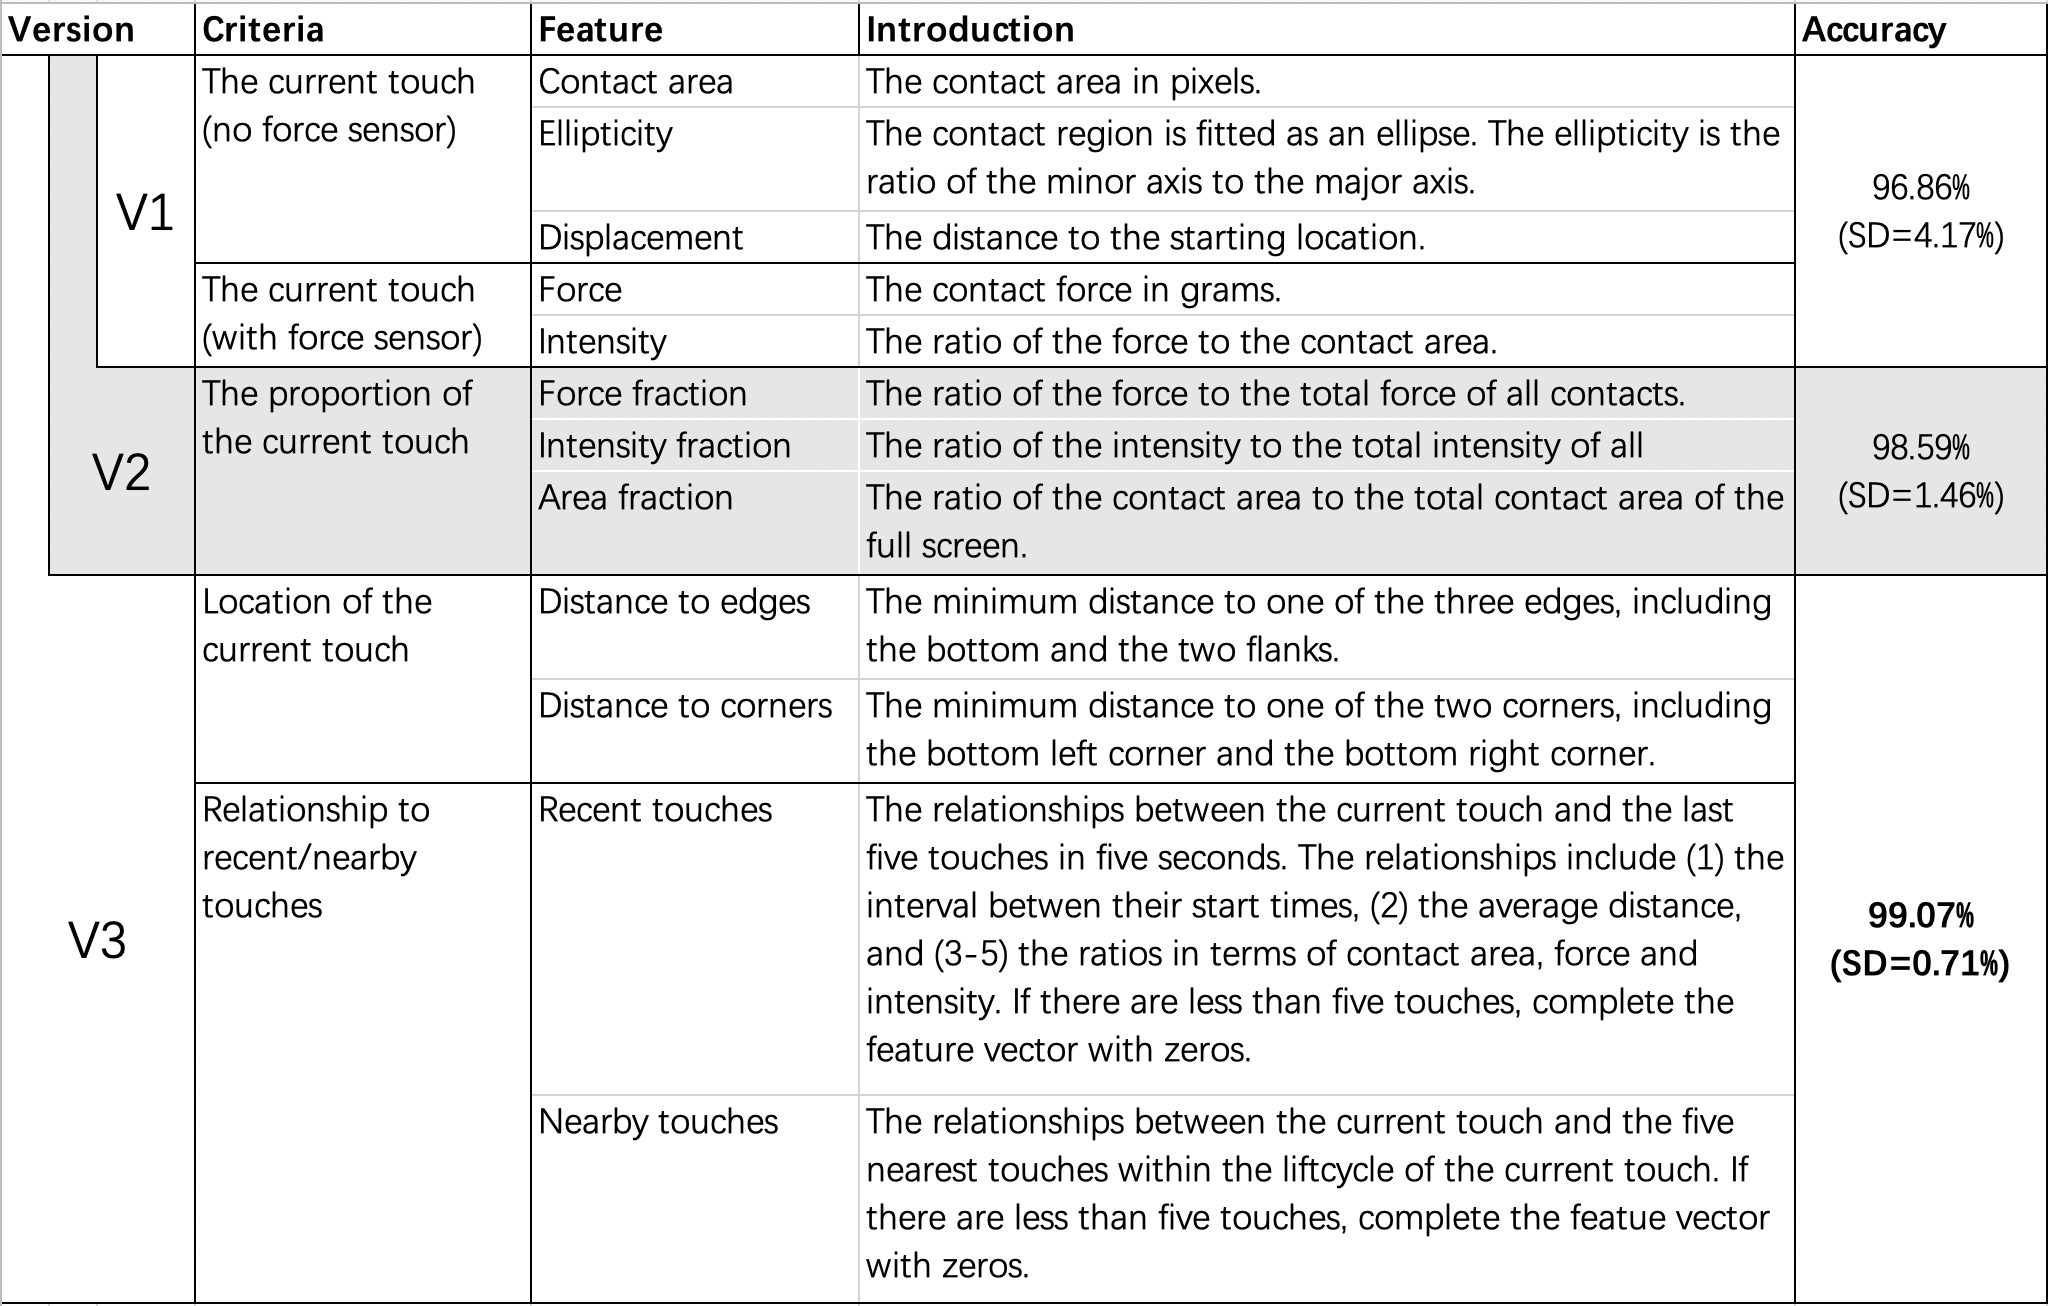
\includegraphics[width=1.0\linewidth]{figures/features.png}
	\centering
	\caption{The features we fed into the SVM model and the accuracy among model versions.}
	\label{fig:feature1}
\end{figure}

【表格:我们的机器学习算法中特征向量的构成】

\subsubsection{Model version 2: filtering out multiple fingers resting}

Observation showed that multiple fingers resting was the most frequent unintentional touches, where users rested more than two fingers on the screen at the same time. There were more than x0\% of multiple finger resting among all unintentional touches. Thus, we add a series of features in the model version 2 to deal with this user behavior. A new criterion was added in the model, namely "the proportion of this touch among all touches". The features in details can be found in table xx (V2). Leave one out cross-validation shows that the accuracy increased to 98.59\%.

% 观察发现,多指同时休息是最常见的误触行为,占所有无意报点总数的x0\%以上。为了解决这个瓶颈问题,我们在模型中新增了一系列表达“本次点击在所有点击中所在的比重”的特征(table xx - V2),这些特征包含本次点击的接触面积、压力和压强占全屏总接触面积、总压力和总压强的比例。对于这三个数值,同样需要计算时域信息,即五帧中的最大值、最小值、平均值、偏度和峰度,共新增15维特征。重新训练得到新的模型(版本2),留一法显示准确率上升至98.59\%。

\subsubsection{Model version 3: understand user behavior and  improve the model}

To understand the user behavior and further improve the model, we analyzed the fail cases of the model version 2. As table xx shows, the error rate of model version 2 was 1.41\%, including xx.x\% false triggering touchpoints and xx.x\% unrecognized touchpoints. We classified the fail cases into 16 categories. We counted their frequencies, analyzed the reasons, and gave possible solutions.

For the fail cases with a white background (xx.x\%) in table xx, the researchers could predict correctly without watching the experiment screencast. That is, the machine should have predicted correctly if it is as smart as a human. For these cases, we proposed features to improve the model. Here are some examples:

%为了进一步提高模型的预测准确率,我们分析了V2版本模型的错例,并推测这些错例是由怎样用户行为导致的。如表格xx所示,有xx.x\%的错例(白色背景部分)是人类(实验者)能够人工分析出正确结果的,我们可以为这些错例设计针对性的特征,从而提高模型的预测准确率。这些错例中比较典型的例子有:

\begin{enumerate}
	\item{\textbf{EG1):} \emph{Hypothenar eminence.} As figure xx.x shows, the hypothenar eminence refers to a group of muscles of the palm that control the motion of the little finger, while the thenar eminence is the group of muscles on the palm at the base of the thumb. Both the two eminences may contact the touchscreen when a user is typing. However, the touches caused by the posiform is usually heavy and intensive, which is easy to confused with intentional touches. Furtunately, these touches are frequently in the bottom left and the bottom right corners. Thus, the distances to the corners could be good features to reject these unintentional touches.}
	\item{\textbf{EG2):} \emph{Continuous touches.} When a user continuously typed on the same key (e.g., the delete key), the follow-up touches might be lighter. 显著性分析发现,连续点击中的后续点击的平均力度为xx.xg,显著低于非后续有意点击的平均水平xx.xg(F,p). These touches are lighter than other intentional touches, so they are likely to be recognized as unintentional touches. Adding information of recent touches could help to correct this fail case.}
	\item{\textbf{EG3):} \emph{One-hand typing.} Some participants typed with one hand, while resting the other hand on the touchsreen. In this situation, the model might think that all the touches together was the "multiple fingers resting" behavior, and identified the case as an unintentional touch. To correct this fail case, we added information of nearby touches, because the typing finger is usually far away from the resting fingers.}
\end{enumerate}

\begin{figure}[!tbh]
	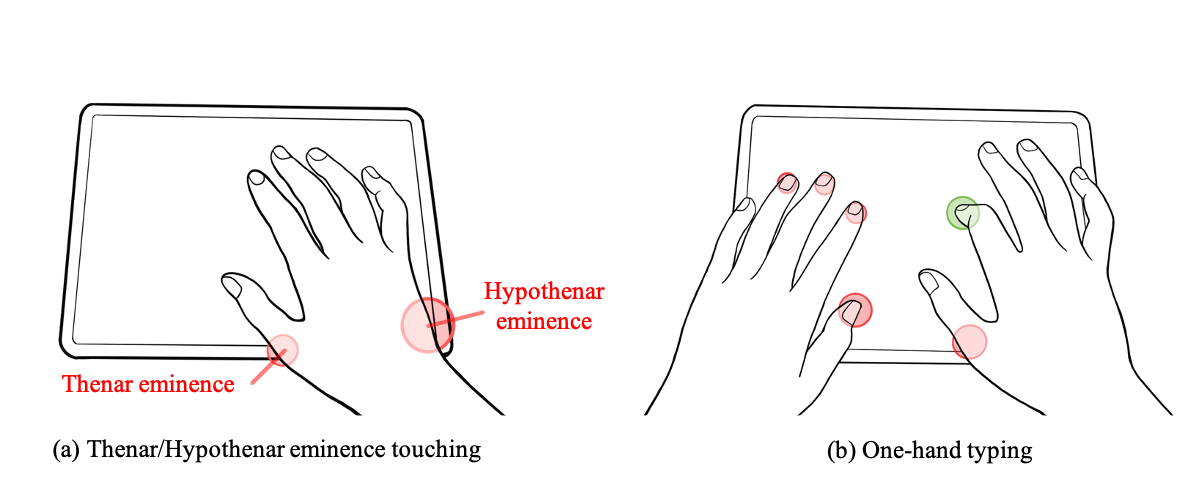
\includegraphics[width=1.0\linewidth]{figures/fail_case_examples.png}
	\centering
	\caption{Fail cases的一些图例.}
	\label{fig:fail_case_examples}
\end{figure}

%(1)V2版模型有些时候会把小鱼际的误触判定为有意点击。我们发现,用户的小鱼际误触主要集中在触摸屏的左下角和右下角。因此,我们给模型添加上了一系列"Distance-to-corners"的特征,这样一来,模型将会降低在小鱼际处识别出有意点击的概率。
%(2)用户在连续点击同一个按键时(比较常见的是删除键),后续的点击可能会变得很轻,使得它的力度看上去更像是一个无意点击,V2版模型不能很好地处理这个问题。因此,我们给模型添加上了一系列"ralationship-to-recent-touches"的特征,这样一来,连续点击即使变得更轻,也能被正确地识别成有意点击。
%(3)有的用户可能会出现单手打字,另一只手指放在屏幕上休息的行为,这种情况下V2版模型可能认为所有手指都是在参与多指休息。因此,我们给模型添加上了一系列"ralationship-to-recent-touches"的特征,这样一来,如果本次点击距离同屏的其它点击距离较远,则可解释为one-hand-typing行为,从而被正确识别为有意点击。

However, there are xx.x\% of the fail cases (with a gray background in table xx), that humans (the researchers) could not predict without watching the experiment screencast. We deemed that these fail cases were inevitable, because the machine can not know what the user is going to enter in advanced. Here are some examples. First, sometimes the participants rested one finger on the touchscreen heavily, which is indistinguishable with a intentional touch. Second, some participants performed a very light touch during entering a word, which is similar to an unintentional touch. That is, the accuracy of the model has an certain upper limit (roughly xx.x\% in this dataset), while our goal is to approach it.

%然而,有xx.x\%的数据(灰色背景部分),是人类也不能在不看上下文(实验录屏)的情况下分析出正确结果的,我们认为这部分的误触和漏报是不可避免的。这一类错例的典型例子有:(1)一只手指休息在键盘上,且力量很大,这种行为和用户打单词的第一个字母的行为非常相似(2)打字过程中出现一次很轻的有意点击,这种行为和打字过程中的误触非常类似。我们认为系统无法避免这种误触,也就是说,即使是人工判断每次点击是否有意,错误率也不低于xx.x\%(V2错误率 * V2错例中人类无法分辨的部分)。

According to the user behaviors summarized in table xx, we added two criteria in the model training. The first criterion is the location of touch, including the minimum distances to the edges and to the corners. The model did not leverage the priori knowledge of the keyboard layout, because the layout of a software keyboard is changeable, while we wanted a universal model. The second criterion is the relationships between the current touch and the recent/nearby touches.The features in details can be found in the table. The model version 3 used all the features listed in table xx. We concentrated these features to form a vector of 100 dimensions and trained an SVM binary classifier. Leave one out cross-validation showed that the accuracy was 99.07\%. The error rate was 0.93\%, including xx.x\% false triggering and xx.x\% unrecognized touchpoints.

We used previous work as baseline \cite{2013-TapBoard}, where every touches that last for more than 450 ms or move father than 15 mm are identified as unintentional touches. We adjusted the thresholds to xx ms and xx mm so that the baseline performed the best on our dataset. Our result (99.07\%) surpassed the baseline (xx.xx\%). In real use, our system calls the classifier once a touch has lasted for five frames or is released in advanced. The system reports the touchpoint if the prediction result is positive. The delay of our method is 100 ms. For comparison, the baseline can only judge a touch when it is released.

%99.07\%的识别准确率远远超过了先前工作[xx]对打字过程中误触的识别准确率,在我们的数据集下,先前工作所使用的阈值方法(时间<xxms,位移<xx厘米)准确率仅为xx.x\%,即使重新调整阈值使其在我们的数据集下达到最优(时间<xxms,位移<xx厘米),准确率也仅为xx.x\%,因此我们的算法在准确率上成倍地提高了已有工作的水平。In real use, the system calls this classifier once a touch is released or has lasted for five frames, and reports the touchpoint if the prediction is positive. The delay is within 100ms. 延迟问题也是我们的算法对比于baseline的一大改进,相比之下,baseline只能在点击事件抬起时做出判断。

%针对表格xx中总结出来的用户行为,我们在模型中新增了两大类特征,分别是本次点击的坐标(V3)和本次点击与时空临近点击之间的关系(V4),最终,新模型的预测准确率达到了99.07\%,十分接近人类判断的准确率。至此,我们认为已经得到了实验一数据下的最佳结果。

\begin{figure}[!tbh]
	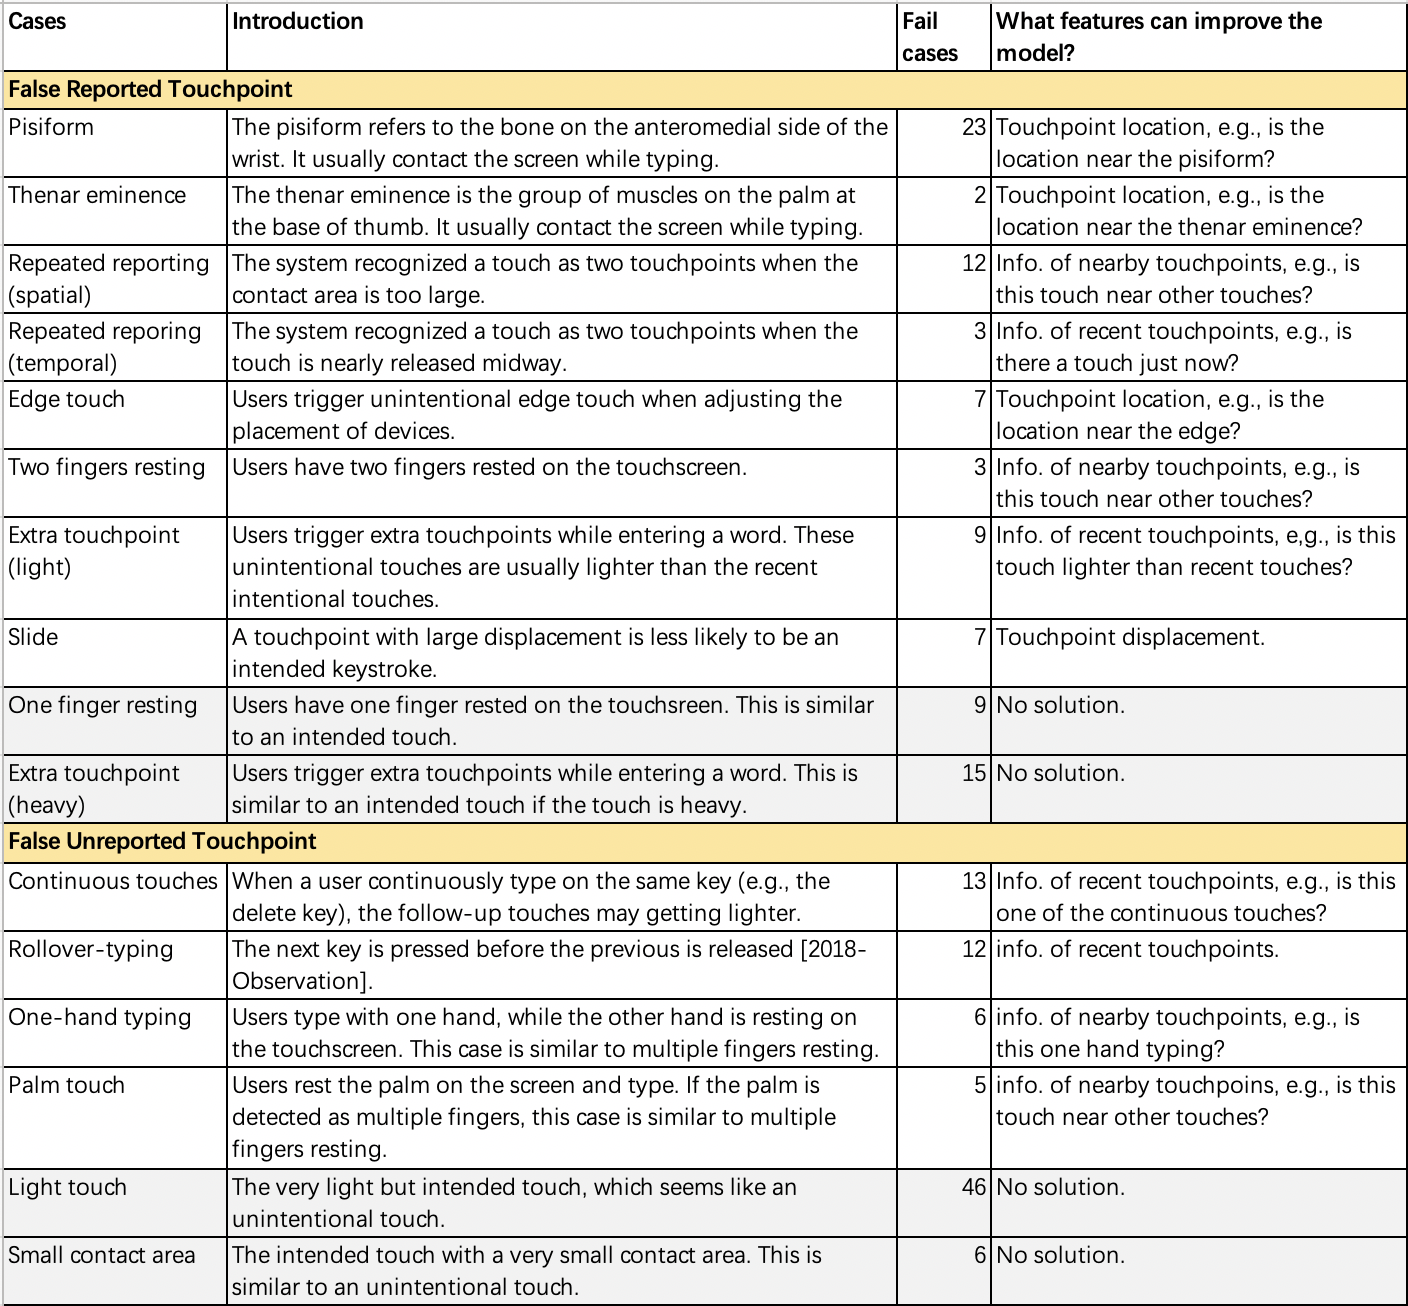
\includegraphics[width=1.0\linewidth]{figures/fail_cases.png}
	\centering
	\caption{Fail cases of the model version 2. Noticed that the "Fail cases" is the number of fail cases of the model, but not a counting for the user behavior. xxx.}
	\label{fig:fail_cases}
\end{figure}

【表格:我们的机器学习算法的fail cases有哪些,解决方法是什么】

We have three conclusions in this experiments. First, participants were willing to rest their fingers on the touchscreen that can reject unintentional touches in imaginary. Hereby, we proposed a hypothesis to be verified, where users are willing to rest their fingers on a real TypeBoard. Second, the force signal is important for rejecting unintentional touches in the text entry task. Third, most unintentional touches (>99\%) can be identified by spatial-temporal features of the signals on a force-sensitive touchsreen keyboard.

%在本实验中,我们能得到三个基本结论:(1)在想象中可以防误触的键盘上,用户十分乐意将手指休息在触屏上。由此我们提出一个假设:如果实际上存在一个能够极大概率拒绝误触,用户也会乐意将手指休息在触屏上。我们会在后续的实验中验证该假设。(2)压力信息对tablets打字防误触算法的提高是显著的。(3)大部分典型的误触行为都可以根据压力屏上触点的时空特性识别出来,准确率超过99\%。除了以上基本结论外,我们还讨论了下列问题:

\subsection{Discussion}

\subsubsection{Why sample five frames in each touch?} There is a trade-off between the amount of sampling frames and the accuracy. The more data we sample in each touch, the more accuracy the prediction is. However, a long sampling window means a large delay, which affects the user experience. We needed to strike a balance. Five frames of sampling results in an acceptable prediction accuracy (99.07\%), meanwhile the delay of 100ms is not perceivable in the touching task [xx].

%为什么选取报点后5帧的数据?首先做出判断的时间和准确率是tradeoff,延迟越大,机器学习的准确率就越高,但同时用户体验受到延迟的影响就越大。为了找到一个平衡点,我们分析了延迟为3帧~7帧的情况,结果如图xx所示,xxx。考虑到用户在点击时能感知到100ms的延迟[xx],我们选取了5帧(100ms)作为算法的判定时机。

\subsubsection{What we found about user behavior?} Here are some conclusions. First, the unintentional touches mainly contains three categories, including multiple fingers resting (xx.x\%), palm touches (xx.x\%) and others (mostly mistaken touches during input, xx.x\%). Second, the text entry task has significant effect on the amount of unintentional touches (F, p). Bonferroni-corrected post-hoc tests showed significant differences between the following task pairs: xx-xx (p<), xx-xx (p<), and xx-xx (p<). Thus, we suggest that studies of unintentional touch should consider the variety of task. We will discuss the user behavior in details in the next study, because it is more meaningful to analyze the user behavior on a real TypeBoard.

%用户行为有什么规律?在这里,我们直接给出几个结论:(1)误触点主要由三部分构成,分别是多指休息(占xx.x\%),手掌误触(占xx.x\%)和输入间误触(xx.x\%),还有其它情况如用户主观打错没有纳入统计。(2)不同任务对用户无意点击数量有显著影响,其中有差异的任务对有xx,这说明,相关工作中讨论不分任务地讨论误触问题是存在问题的。我们不对以上规律作展开讨论,因为实验一采集的是用户在想象中的防误触键盘上的打字数据,该数据的代表性不强。在下一个实验当中,我们将会采集用户在model-version-4上的打字行为,迭代式地继续改进误触识别算法,并更加详细地探讨用户的行为。
